\subsubsection{UC\theuccount-PG - GitLab segnala apertura issue al Producer GitLab}
%	\begin{figure}[H]
%		\centering
%		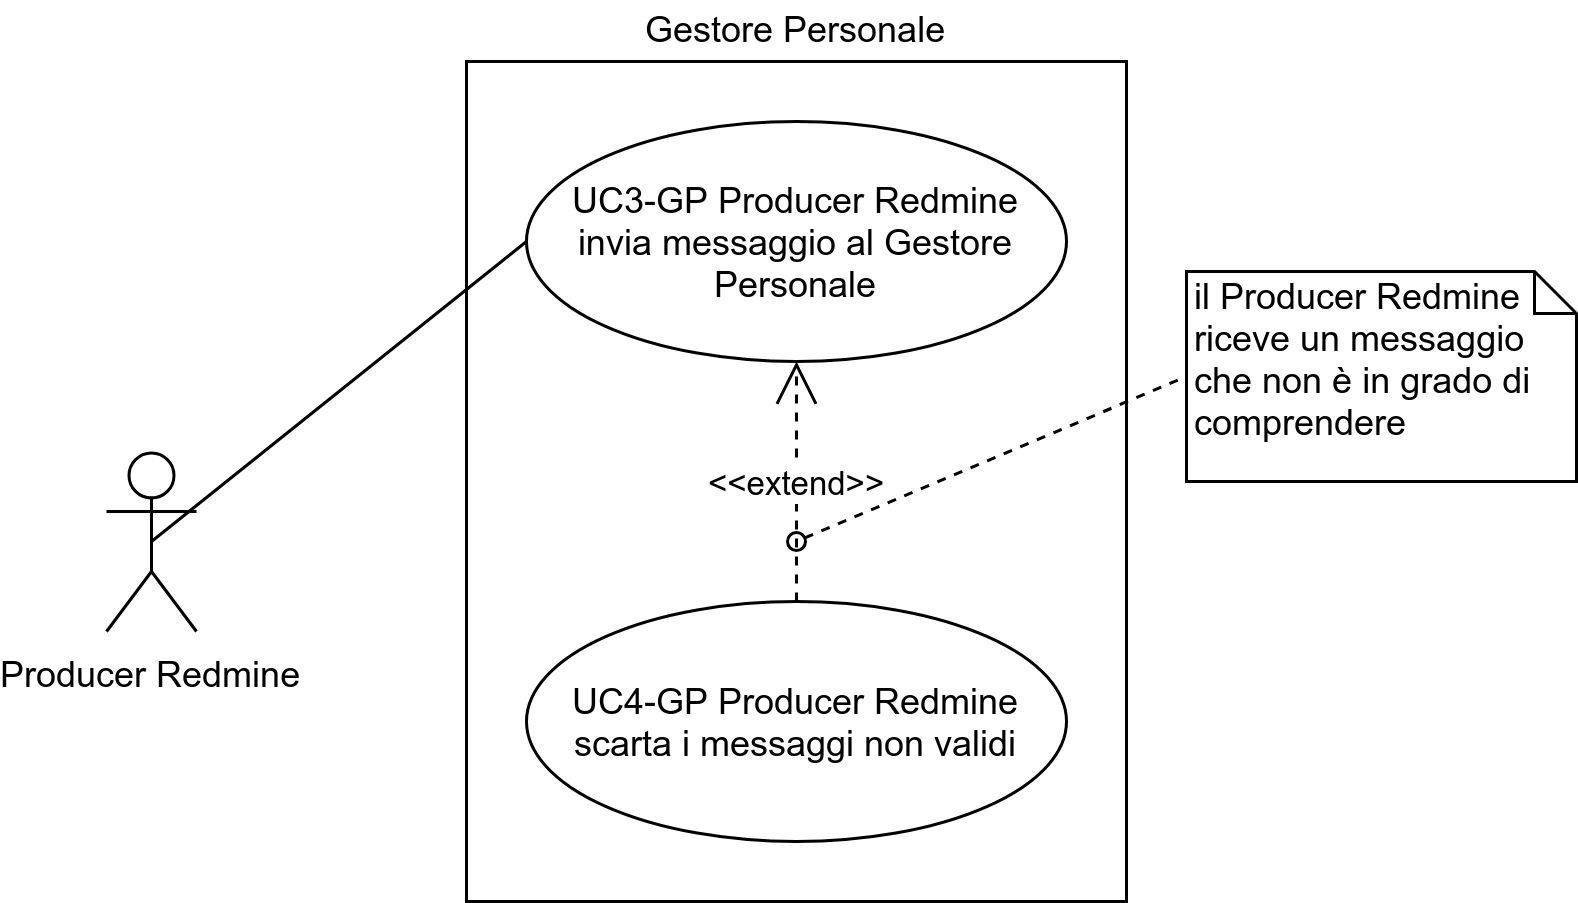
\includegraphics[width=0.5\textwidth]{img/casi_d'uso/UC4.png}\\
%		\caption{UC\theuccount-PG - GitLab segnala apertura issue al Producer GitLab}
%	\end{figure}
	\begin{itemize}
		\item \textbf{Codice}: UC\theuccount-PG.
		\item \textbf{Titolo}: GitLab segnala apertura issue al Producer GitLab.
		\item \textbf{Attori primari}: GitLab.
		\item \textbf{Descrizione}: GitLab segnala l'apertura di una nuova issue tramite webhook a \progetto.
		L'apertura di una issue su GitLab contiene:
		\begin{itemize}
			\item Object kind
			\item Action
			\item Title e opzionalmente:
			\begin{itemize}
				\item Label
				\item Milestone
				\item Assignees
				\item Due Date
			\end{itemize}
		\end{itemize}
		Il campo object kind ci permette di capire il tipo di oggetto, in questo caso infatti contiene ``issue'', mentre il campo action ha ``open''.
		\item \textbf{Precondizione}: viene aperta una issue su GitLab da 
		segnalare a \progetto.
		\item \textbf{Postcondizione}: il Producer GitLab riceve la segnalazione da GitLab.
		\item \textbf{Scenario principale}: 
		\begin{enumerate}
			\item Viene aperta una nuova issue su GitLab
			\item GitLab procede all'invio della segnalazione di issue al Producer GitLab
		\end{enumerate}
		
	\end{itemize}